\documentclass{article}
\usepackage{graphicx}
\usepackage[dvipsnames,table]{xcolor}
\usepackage[utf8]{inputenc}
\usepackage{siunitx}
\usepackage[american,siunitx]{circuitikz}
\usepackage{amsmath}
\usepackage{svg}
\usepackage{booktabs}
\usepackage{float}
\usepackage{xparse, xfp}
\usepackage{multirow}
\usepackage{tikz}
\usepackage{karnaugh-map}
\usepackage{pdfpages}
\usepackage{hyperref}
\hypersetup{
    colorlinks=true,
    linkcolor=blue,
    filecolor=magenta,      
    urlcolor=cyan,
}
\usetikzlibrary{calc}
%\usepackage[landscape]{geometry}
\renewcommand{\thesubsection}{\thesection.\alph{subsection}}
\newcommand{\equal}{=}
\newcommand{\greyrule}{\arrayrulecolor{black!30}\midrule\arrayrulecolor{black}}
\makeatletter
\newcommand\currcoor{\the\tikz@lastxsaved,\the\tikz@lastysaved}
\makeatother
\newcolumntype{:}{@{\hskip\tabcolsep\color{black!30}\vrule\hskip\tabcolsep}}

\ExplSyntaxOn
\NewExpandableDocumentCommand \groupify { O{\,\allowbreak} m m }
  { \jakob_groupify:nnn {#1} {#2} {#3} }
\cs_new:Npn \jakob_groupify:nnn #1 #2 #3
  { \__jakob_groupify_loop:nnw { 1 } {#2} #3 \q_recursion_tail {#1} \q_recursion_stop }
\cs_new:Npn \__jakob_groupify_loop:nnw #1 #2 #3
  {
    \quark_if_recursion_tail_stop:n {#3}
    \exp_not:n {#3}
    \int_compare:nNnTF {#1} = {#2}
      { \__jakob_groupify_sep:n }
      { \exp_args:Nf \__jakob_groupify_loop:nnw { \int_eval:n { #1+1 } } }
          {#2}
  }
\cs_new:Npn \__jakob_groupify_sep:n #1 #2 \q_recursion_tail #3
  {
    \tl_if_empty:nF {#2} { \exp_not:n {#3} }
    \__jakob_groupify_loop:nnw { 1 } {#1}
    #2 \q_recursion_tail {#3}
  }
\ExplSyntaxOff

\title{ECE 2200L\\Introduction to Microelectronics Circuits Laboratory\\\,\\Experiment 1\\AC Frequency Response Test\\\,\\Report}
\author{Choi Tim Antony Yung}
\begin{document}
\maketitle

\thispagestyle{empty}
\setcounter{page}{0}

\newpage

\section*{Objective}

The objective of this emperiment is to familiarize the operation and usage of Excel and Spice and to compare the theoretical result obtained from Excel and Spice to the experimental result obtained from the physical circuit.

\section*{Procedure}
The following circuit was simulated in PSpice.
\begin{figure}[H]
  \centering
  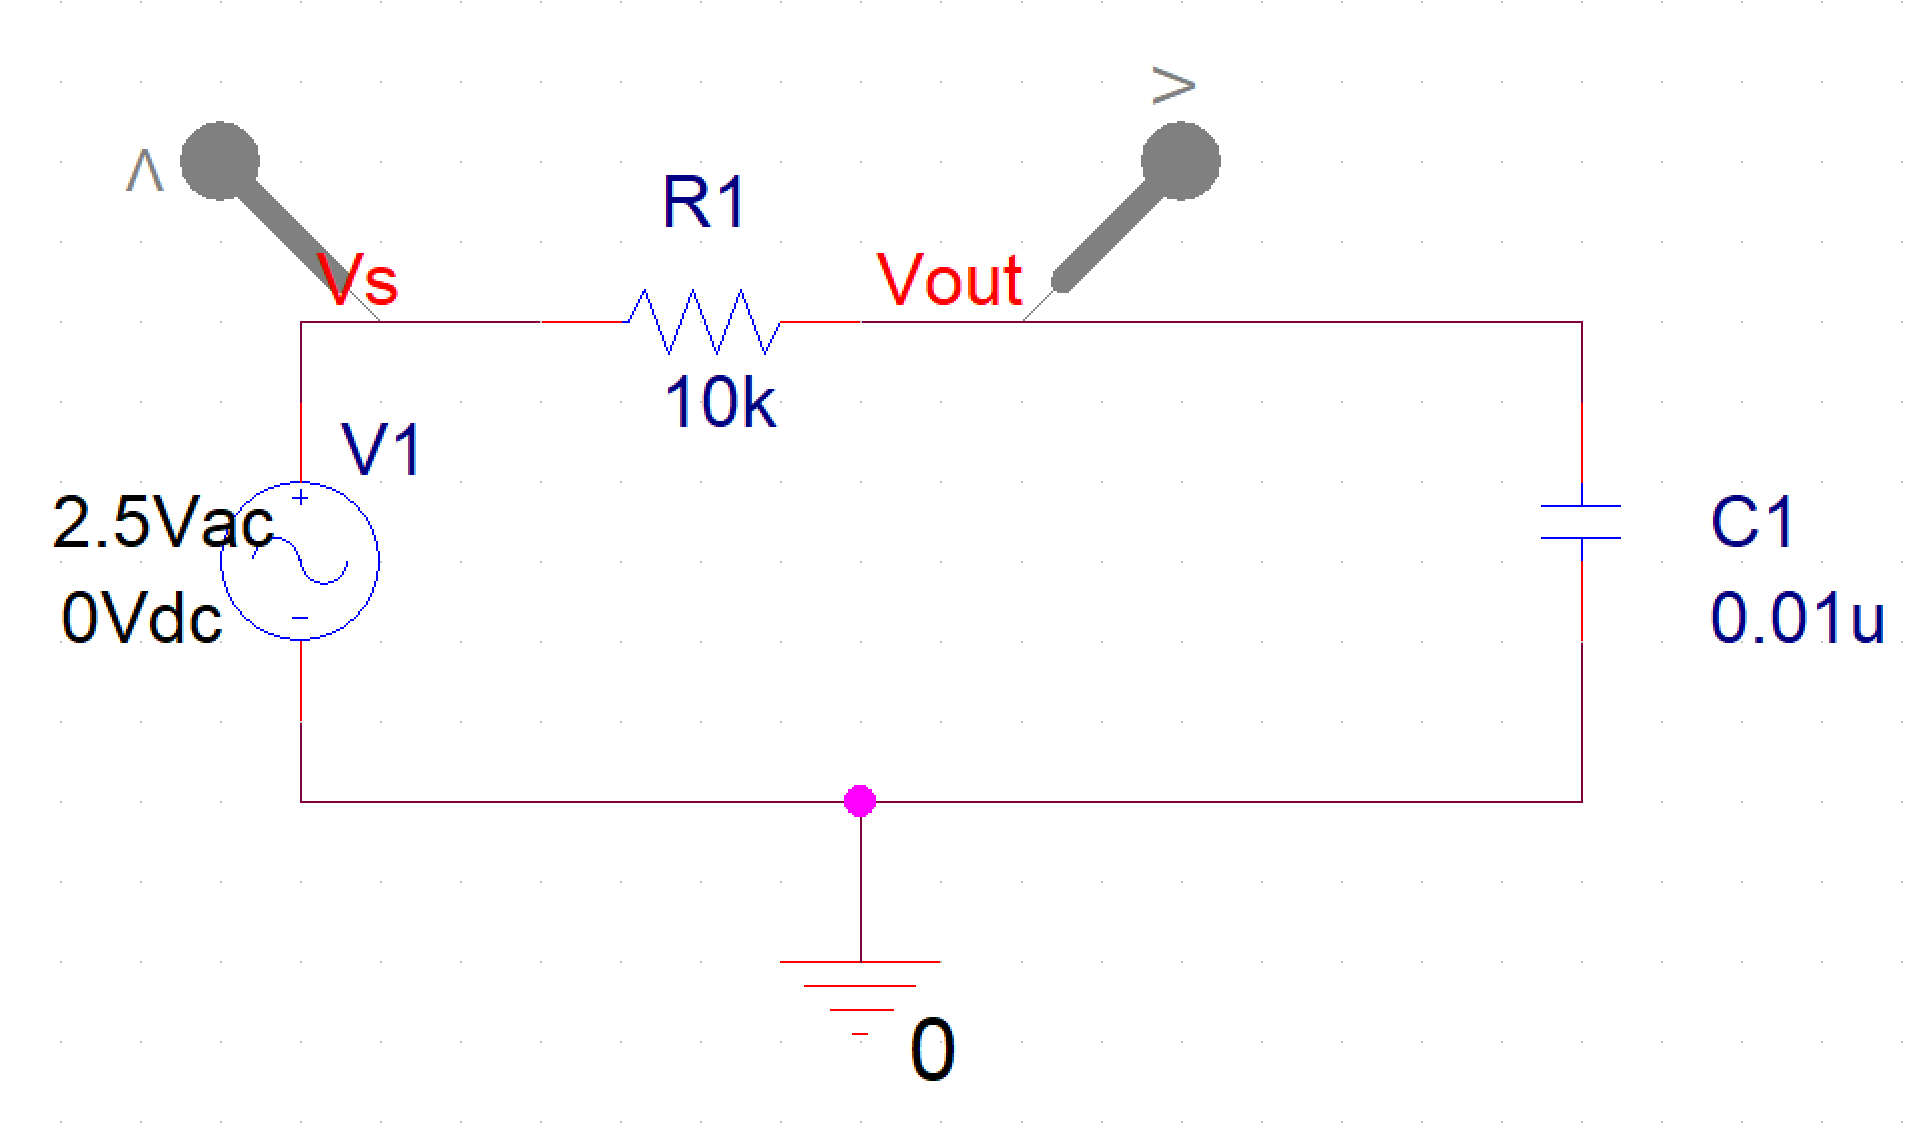
\includegraphics[width=\textwidth]{ECE2200_Lab1_pspice_schematic.png}
\end{figure}
\section*{Result}
The following is the experimental data obtained from the physical circuit.
\begin{table}[H]
  \begin{tabular}{r|ccccccc}
      \toprule
      Frequency $\mathit{f}$ (kHz) & 0.1 & 0.3 & 1 & 3 & 10 & 30 & 100\\
      \midrule
      Vout$_{pp}$ (V)& 5.0 & 4.9 & 4.3 & 2.49 & 0.88 & 0.334 & 0.155 \\
      $20log\frac{V_{out}}{V_{S}}$ (dB)& 0 & -0.17 & -1.3 & -6.1 & -15.1 & -23.5 & -30 \\
      $\theta$ ($^\circ$)& -3 & -11 & -31 & -61 & -82 & -87 & -89 \\
      \bottomrule
  \end{tabular}
\end{table}
\begin{figure}[H]
  \centering
  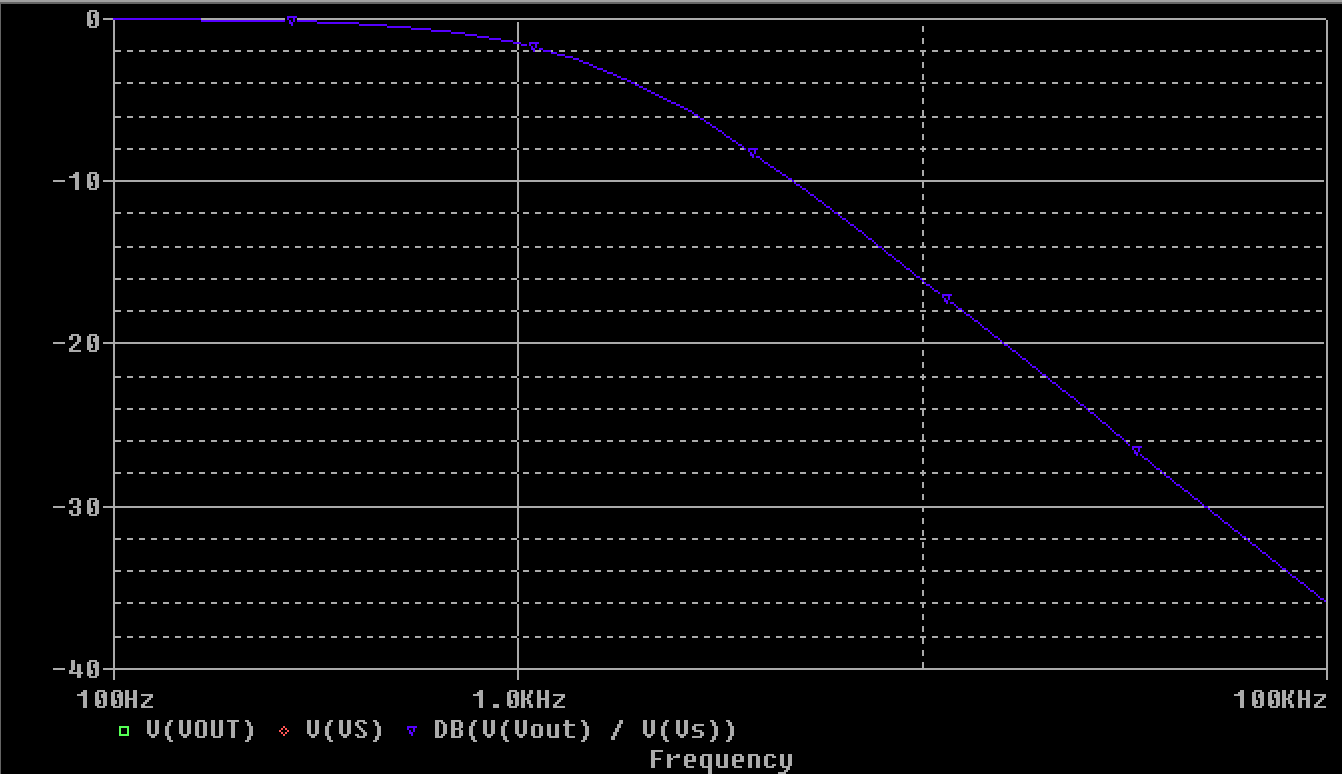
\includegraphics[width=\textwidth]{ECE2200_Lab1_pspice.png}
  \caption{Mag[T(jf)] in dB vs. Frequency in Hz plot from PSpice simulation}
\end{figure}
\begin{figure}[H]
  \centering
  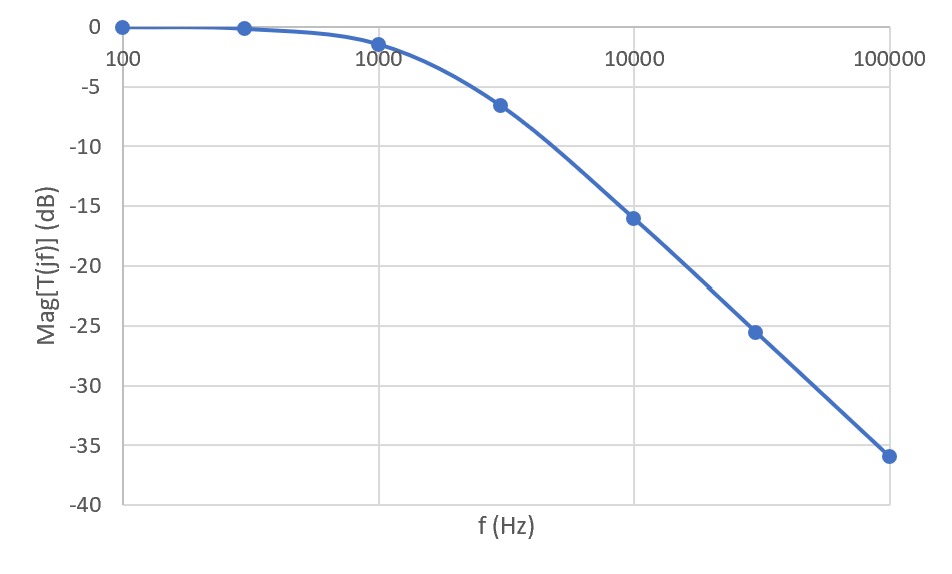
\includegraphics[width=\textwidth]{ECE2200_Lab1_excel.png}
  \caption{Mag[T(jf)] in dB vs. Frequency in Hz plot from theoretical data points in Excel}
\end{figure}
\begin{figure}[H]
  \centering
  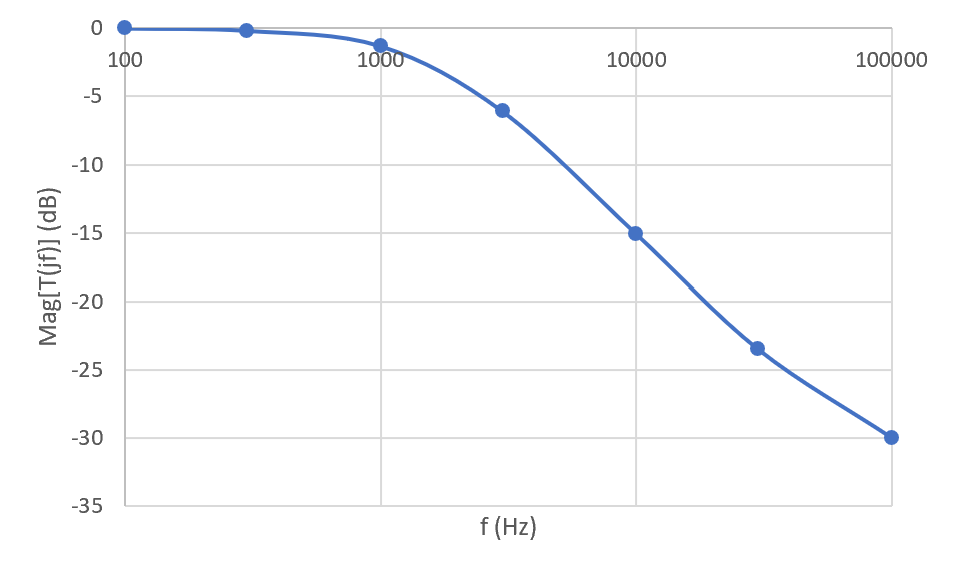
\includegraphics[width=\textwidth]{ECE2200_Lab1_excel_exp.png}
  \caption{Mag[T(jf)] in dB vs. Frequency in Hz plot from experimental data points in Excel}
\end{figure}
\begin{figure}[H]
  \centering
  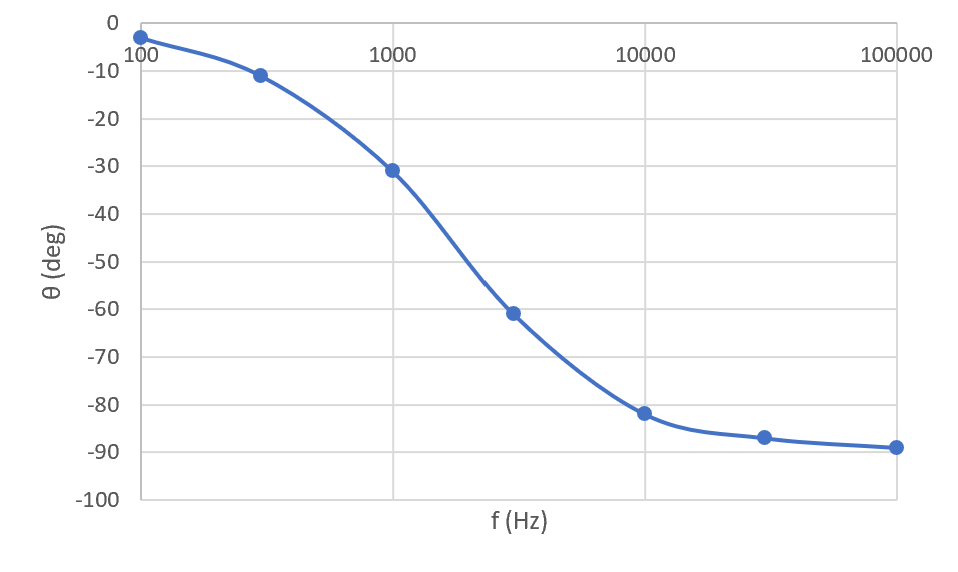
\includegraphics[width=\textwidth]{ECE2200_Lab1_excel_theta.png}
  \caption{$\theta$ in $^\circ$ vs. Frequency in Hz plot from experimental data points in Excel}
\end{figure}

\pagebreak

\section*{Conclusion}
As can be seen in the previous chart, the plot derived from the theoretical dataset is almost identical to the plot generated by PSpice from the circuit simulation. However, the plot of gain generated from the experimental result is somewhat skewed upward when comparing to the plot generated from the theoretical result. The noise in the measurement could be a contributing factor since it would drown the output voltage when it is small to make it appears to be higher than it is, hence the upward skew affecting more severely when the frequency is higher and the output voltage is lower.

\end{document}
